% 注意事项:编译两次,以确保目录、页码完整显示

\def\allfiles{}

\documentclass[14pt,a4paper,UTF8,twoside]{article}

% Formatting Packages ——————————————————————————————————————
\usepackage{multicol}
\usepackage{multirow}
\usepackage{enumitem}
\usepackage{indentfirst}
\usepackage[toc]{multitoc}

% Math & Physics Packages ————————————————————————————
\usepackage{amsmath, amsthm, amsfonts, amssymb}
\usepackage{setspace}
\usepackage{physics}
\usepackage{cancel}
\usepackage{nicefrac}
\usepackage{unicode-math} % 允许数学公式使用特定字体

% Image-related Packages —————————————————————————————
\usepackage{float} % 浮动体环境
\usepackage{subcaption} % 子图包
\usepackage{graphics, graphicx}
\usepackage{tikz, tikz-qtree}
\usepackage{mdframed}
\usepackage{lmodern}
\usetikzlibrary{arrows.meta}
\usetikzlibrary{shapes.geometric, arrows}
\tikzstyle{startstop} = [rectangle, rounded corners, minimum width=3cm, minimum height=1cm,text centered, draw=black, fill=red!30]
\tikzstyle{process} = [rectangle, minimum width=3cm, minimum height=1cm, text centered, draw=black, fill=blue!30]
\tikzstyle{arrow} = [thick,->,>=stealth]

\usepackage{pgfplots}
\pgfplotsset{compat=1.18}
\usepackage{xcolor}
\usepackage{fourier-orns}
\usepackage{lipsum}

% Colour Palette ——————————————————————————————————————
\definecolor{merah}{HTML}{F4564E}
\definecolor{merahtua}{HTML}{89313E}
\definecolor{biru}{HTML}{60BBE5}
\definecolor{birutua}{HTML}{412F66}
\definecolor{hijau}{HTML}{59CC78}
\definecolor{hijautua}{HTML}{366D5B}
\definecolor{kuning}{HTML}{FFD56B}
\definecolor{jingga}{HTML}{FBA15F}
\definecolor{ungu}{HTML}{8C5FBF}
\definecolor{lavender}{HTML}{CBA5E8}
\definecolor{merjamb}{HTML}{FFB6E0}
\definecolor{mygray}{HTML}{E6E6E6}
\definecolor{mygreen}{rgb}{0,0.6,0}
\definecolor{mymauve}{rgb}{0.58,0,0.82}

% Theorems ————————————————————————————————————————————
\usepackage{tcolorbox}
\usepackage{changepage}
\tcbuselibrary{skins,breakable,theorems}

\newcounter{hitung}
\setcounter{hitung}{\thesection}

\makeatletter
	% Proof 证明如下
	\def\tcb@theo@widetitle#1#2#3{\hbox to \textwidth{\textsc{\large#1}\normalsize\space#3\hfil(#2)}}
	\tcbset{
		theorem style/theorem wide name and number/.code={ \let\tcb@theo@title=\tcb@theo@widetitle},
		proofbox/.style={skin=enhancedmiddle,breakable,parbox=false,boxrule=0mm,
			check odd page, toggle left and right, colframe=black!20!white!92!hijau,
			leftrule=8pt, rightrule=0mm, boxsep=0mm,arc=0mm, outer arc=0mm,
			left=3mm,right=3mm,top=0mm,bottom=0mm, toptitle=0mm,
			bottomtitle=0mm,colback=gray!3!white!98!biru, before skip=8pt, after skip=8pt,
			before={\par\vskip-2pt},after={\par\smallbreak},
		},
	}
	\newtcolorbox{ProofBox}{proofbox}
	\makeatother
	
	\let\realproof\proof
	\let\realendproof\endproof
	\renewenvironment{proof}[1][Prove:]{\ProofBox\strut\textsc{#1}\space}{\endProofBox}
        \AtEndEnvironment{proof}{\null\hfill$\blacksquare$}
        % Definition 定义环境
	\newtcbtheorem[use counter=hitung, number within=section]{dfn}{定义}
	{theorem style=theorem wide name and number,breakable,enhanced,arc=3.5mm,outer arc=3.5mm,
		boxrule=0pt,toprule=1pt,leftrule=0pt,bottomrule=1pt, rightrule=0pt,left=0.2cm,right=0.2cm,
		titlerule=0.5em,toptitle=0.1cm,bottomtitle=-0.1cm,top=0.2cm,
		colframe=white!10!biru,
		colback=white!90!biru,
		coltitle=white,
		shadow={1.3mm}{-1.3mm}{0mm}{gray!50!white}, % 添加阴影
        coltext=birutua!60!gray, title style={white!10!biru}, rbefoe skip=8pt, after skip=8pt,
		fonttitle=\bfseries,fontupper=\normalsize}{dfn}

	% 答题卡
	\newtcbtheorem[use counter=hitung, number within=section]{ans}{解答}
	{theorem style=theorem wide name and number,breakable,enhanced,arc=3.5mm,outer arc=3.5mm,
		boxrule=0pt,toprule=1pt,leftrule=0pt,bottomrule=1pt, rightrule=0pt,left=0.2cm,right=0.2cm,
		titlerule=0.5em,toptitle=0.1cm,bottomtitle=-0.1cm,top=0.2cm,
		colframe=white!10!biru,
		colback=white!90!biru,
		coltitle=white,
		shadow={1.3mm}{-1.3mm}{0mm}{gray!50!white}, % 添加阴影
        coltext=birutua!60!gray, title style={white!10!biru}, before skip=8pt, after skip=8pt,
		fonttitle=\bfseries,fontupper=\normalsize}{ans}

	% Axiom
	\newtcbtheorem[use counter=hitung, number within=section]{axm}{公理}
	{theorem style=theorem wide name and number,breakable,enhanced,arc=3.5mm,outer arc=3.5mm,
		boxrule=0pt,toprule=1pt,leftrule=0pt,bottomrule=1pt, rightrule=0pt,left=0.2cm,right=0.2cm,
		titlerule=0.5em,toptitle=0.1cm,bottomtitle=-0.1cm,top=0.2cm,
		colframe=white!10!biru,colback=white!90!biru,coltitle=white,
		shadow={1.3mm}{-1.3mm}{0mm}{gray!50!white!90}, % 添加阴影
        coltext=birutua!60!gray,title style={white!10!biru},before skip=8pt, after skip=8pt,
		fonttitle=\bfseries,fontupper=\normalsize}{axm}
 
	% Theorem
	\newtcbtheorem[use counter=hitung, number within=section]{thm}{定理}
	{theorem style=theorem wide name and number,breakable,enhanced,arc=3.5mm,outer arc=3.5mm,
		boxrule=0pt,toprule=1pt,leftrule=0pt,bottomrule=1pt, rightrule=0pt,left=0.2cm,right=0.2cm,
		titlerule=0.5em,toptitle=0.1cm,bottomtitle=-0.1cm,top=0.2cm,
		colframe=white!10!merah,colback=white!75!pink,coltitle=white, coltext=merahtua!80!merah,
		shadow={1.3mm}{-1.3mm}{0mm}{gray!50!white!90}, % 添加阴影
		title style={white!10!merah}, before skip=8pt, after skip=8pt,
		fonttitle=\bfseries,fontupper=\normalsize}{thm}
	
	% Proposition
	\newtcbtheorem[use counter=hitung, number within=section]{prp}{命题}
	{theorem style=theorem wide name and number,breakable,enhanced,arc=3.5mm,outer arc=3.5mm,
		boxrule=0pt,toprule=1pt,leftrule=0pt,bottomrule=1pt, rightrule=0pt,left=0.2cm,right=0.2cm,
		titlerule=0.5em,toptitle=0.1cm,bottomtitle=-0.1cm,top=0.2cm,
		colframe=white!10!hijau,colback=white!90!hijau,coltitle=white, coltext=hijautua!80!brown,
		shadow={1.3mm}{-1.3mm}{0mm}{gray!50!white}, % 添加阴影
		title style={white!10!hijau}, before skip=8pt, after skip=8pt,
		fonttitle=\bfseries,fontupper=\normalsize}{prp}


	% Example
	\newtcolorbox[use counter=hitung, number within=section]{cth}[1][]{breakable,
		colframe=white!10!jingga, coltitle=white!90!jingga, colback=white!85!jingga, coltext=black!10!brown!50!jingga, colbacktitle=white!10!jingga, enhanced, fonttitle=\bfseries,fontupper=\normalsize, attach boxed title to top left={yshift=-2mm}, before skip=8pt, after skip=8pt,
		title=Itemize~\thetcbcounter \ \ #1}

	% Catatan/Note
	\newtcolorbox{ctt}[1][]{enhanced, 
		left=4.1mm, borderline west={8pt}{0pt}{white!10!kuning}, 
		before skip=6pt, after skip=6pt, 
		colback=white!85!kuning, colframe= white!85!kuning, coltitle=orange!60!kuning!25!brown, coltext=orange!60!kuning!25!brown,
		fonttitle=\bfseries,fontupper=\normalsize, before skip=8pt, after skip=8pt,
		title=\underline{Notice}  #1}
	
	% Komentar/Remark
	\newtcolorbox{rmr}[1][]{
		,arc=0mm,outer arc=0mm,
		boxrule=0pt,toprule=1pt,leftrule=0pt,bottomrule=5pt, rightrule=0pt,left=0.2cm,right=0.2cm,
		titlerule=0.5em,toptitle=0.1cm,bottomtitle=-0.1cm,top=0.2cm,
		colframe=white!10!kuning,colback=white!85!kuning,coltitle=white, coltext=orange!60!kuning,
		fonttitle=\bfseries,fontupper=\normalsize, before skip=8pt, after skip=8pt,
		title=Question  #1}

\usepackage{booktabs} % 表格库
\usepackage{titlesec} % 标题库
\usepackage{fancyhdr} % 页眉页脚库
\usepackage[sorting=none]{biblatex}
\usepackage{array}
\usepackage{longtable}
\usetikzlibrary{positioning, arrows.meta}
\addbibresource{references.bib} % 指定你的.bib文件名称

\date{} % 留空,以让编译时去除日期

%———————————————注意事项—————————————————%

% 1、如果编译显示失败,但没有错误信息,就是 filename.pdf 正在被占用
% 2、在文件夹中的终端使用 Windows > xelatex filename.tex 也可编译

%—————————————华东师范大学———————————————%

% 论文制作时须加页眉,页眉从中文摘要开始至论文末
% 偶数页码内容为:华东师范大学硕士学位论文,奇数页码内容为学位论文题目

%————————定义 \section 的标题样式————————%

% 注意:\chapter 等命令,内部使用的是 \thispagestyle{plain} 的排版格式
% 若需要自己加上页眉,实际是在用 \thispagestyle{fancy} 的排版格式
% 加上下面这一段指令,就能够让 \section 也使用 fancy 的排版格式
% 本质就是让目录、第一页也能够显示页眉、页脚

\fancypagestyle{plain}{
  \pagestyle{fancy}
}

\title{华东师范大学软件学院实验报告} % 模板
\titleformat{\section}
    {\normalfont\bfseries\Large} % 字体大小、字体系列(\bfseries 为加粗)
    {\thesection}{1em}{}

% ———————————设置章节的中文格式———————————%
\renewcommand\thesection{\chinese{section} \hspace{0pt}}
\renewcommand\thesubsection{\arabic{subsection} \hspace{0pt}}
% \renewcommand\thesubsubsection{\alph{subsubsection} \hspace{0pt}} % 字母编号
% \hspace{0pt} 是为了确保在章节编号和章节题目之间不要有空格,使得排版更为美观
    
%—————————————页面基础设置———————————————%

\usepackage{geometry}
\geometry{left=10mm, right=10mm, top=20mm, bottom=20mm}

%————————————设置页眉、页脚——————————————%

\pagestyle{fancy} % 设置 plain style 的属性

% 设置页眉

\fancyhead[RE]{\footnotesize \leftmark} % Right Even 偶数页右侧显示章名 \leftmark 最高级别章名
\fancyhead[LO]{\footnotesize \rightmark} % Left Odd 奇数页左侧显示节名 \rightmark 第二级别节名
\fancyhead[C]{华东师范大学软件学院实验报告} % Center 居中显示
\fancyhead[LE,RO]{~\thepage~} % 在偶数页的左侧,奇数页的右侧显示页码
\renewcommand{\headrulewidth}{1.2pt} % 页眉与正文之间的水平线粗细

% 设置页脚:在每页的右下脚以斜体显示书名

\fancyfoot[RO,RE]{\it Lab Report By \LaTeX} % 使用意大利斜体显示
\renewcommand{\footrulewidth}{0.5pt} % 页脚水平线宽度

%——————设置页码:在底部居中显示页码———————%

\usepackage{lastpage} % 页码数库
\pagestyle{fancy}
\fancyfoot[C]{\kaishu 第 \thepage 页 \ 共 \pageref{LastPage} 页} % LastPage 需要二次编译以获取总页数

%——————————————代码块设置———————————————%

\usepackage{listings} % 代码块包
\lstset {
    backgroundcolor=\color{white},   % choose the background color; you must add \usepackage{color} or \usepackage{xcolor}
    basicstyle=\footnotesize,        % the size of the fonts that are used for the code
    breakatwhitespace=false,         % sets if automatic breaks should only happen at whitespace
    breaklines=true,                 % sets automatic line breaking
    captionpos=bl,                   % sets the caption-position to bottom
    commentstyle=\color{mygreen},    % comment style
    deletekeywords={...},            % if you want to delete keywords from the given language
    escapeinside={\%*}{*},           % if you want to add LaTeX within your code
    extendedchars=true,              % lets you use non-ASCII characters; for 8-bits encodings only, does not work with UTF-8
    frame=single,                    % adds a frame around the code
    keepspaces=true,                 % keeps spaces in text, useful for keeping indentation of code (possibly needs columns=flexible)
    keywordstyle=\color{blue},       % keyword style
    % language=Python,               % the language of the code
    morekeywords={*,...},            % if you want to add more keywords to the set
    numbers=left,                    % where to put the line-numbers; possible values are (none, left, right)
    numbersep=5pt,                   % how far the line-numbers are from the code
    numberstyle=\tiny\color{mygray}, % the style that is used for the line-numbers
    rulecolor=\color{black},         % if not set, the frame-color may be changed on line-breaks within not-black text (e.g. comments (green here))
    showspaces=false,                % show spaces everywhere adding particular underscores; it overrides 'showstringspaces'
    showstringspaces=false,          % underline spaces within strings only
    showtabs=false,                  % show tabs within strings adding particular underscores
    stepnumber=1,                    % the step between two line-numbers. If it's 1, each line will be numbered
    stringstyle=\color{orange},      % string literal style
    tabsize=2,                       % sets default tabsize to 2 spaces
    % title=Python Code              % show the filename of files included with \lstinputlisting; also try caption instead of title
}

% 注释掉的部分用于后续插入代码,参数可调整,格式如下:

% 1、直接插入
% \begin{lstlisting}[language = ? , title = { ? } ]
%       Your code here.
% \end{lstlisting}

% 2、文件插入
% \lstinputlisting[language = C , title = ?.c] {filename.c}

%———————————————字体设置————————————————%

\usepackage{fontspec} % 允许设置字体
\usepackage[utf8]{inputenc}
\usepackage{ctex}
\usepackage{pifont}
\linespread{1.2}
% \setCJKmainfont{SimSun} % 设置正文罗马族的 CJK 字体

%———————————————超链接设置——————————————%

\usepackage[hidelinks]{hyperref}
\hypersetup{
    pdfstartview=FitH, % 设置PDF文档打开时的初始视图为页面宽度适应窗口宽度(即页面水平适应)
    CJKbookmarks=true, % 用对CJK(中文、日文、韩文)字符的书签支持,确保这些字符在书签中正确显示
    bookmarksnumbered=true, % 书签带有章节编号。这对有章节编号的文档很有用
    bookmarksopen=true, % 文档打开时,书签树是展开的,方便查看所有书签
    colorlinks, % 启用彩色链接。这样,链接在PDF中会显示为彩色,而不是默认的方框
    pdfborder=001, % 设置PDF文档中链接的边框样式。001 表示链接周围没有边框,仅在单击时显示一个矩形
    linkcolor=blue, % 设置文档内部链接(如目录中的章节链接)的颜色为蓝色
    anchorcolor=blue, % 设置锚点链接(即目标在同一文档内的链接)的颜色为蓝色
    citecolor=blue, % 设置引用(如文献引用)的颜色为蓝色
}

%————————————导言区结束,进入正文部分————————————%

\begin{document}

\maketitle

\begin{center} % \extracolsep{\fill} 拉伸到页面最大宽度前,保证居中显示

  \begin{tabular*}{\textwidth}{@{\extracolsep{\fill}} l  l  l }
    \hline
    实验课程:计算机网络实践 &  年级:2023级本科  &  实验成绩: \\
    实验名称:Lab 7 Socket Programming & 姓名:张梓卫 \\
    实验编号:(7) & 学号:10235101526 & 实验日期:2025/01/03 \\
    指导老师:刘献忠 & 组号:& 实验时间:2 课时 \\
    \hline
  \end{tabular*}

\end{center}

\tableofcontents % 目录也需要二次编译

\begin{ctt}
    本 PDF 可以点击目录跳转,您可以点击不同位置以获取相关内容。
\end{ctt}

\section{实验目的}

该实验是课程《计算机网络实践》第七次实验,全名《Socket Programming》,目标如下:

\begin{cth}
\begin{itemize}
    \item 熟悉 Socket 编程的基本原理
    \item 掌握简单的套接字编程
    \item 掌握通过 Socket 编程实现 C/S 程序的基本方法
    \item 了解应用层和运输层的作用及相关协议的工作原理和机制    
\end{itemize}
\end{cth}

\section{实验内容与实验步骤}

\subsection{实验要求}

要实现多个 Client 客户端与 Server 服务端之间的 Socket 通信,需要满意以下要求:

\begin{itemize}
    \begin{multicols}{2}

    \item \textbf{Server 端要求}:
    
    \begin{cth}
    \begin{itemize}
        \item 能够将 Client 的输入信息进行标准输出打印;
        \item 支持 5 个以上的 Client 同时发送消息并打印;
        \item 端口号绑定错误时有报错。
    \end{itemize}
    \end{cth} 

    \columnbreak

    \item \textbf{Client 端要求}:
    
    \begin{cth}
    \begin{itemize}
        \item 能从标准输入或文件中接受消息;
        \item 标准输入以 \textbf{两个回车} 作为结束标志;
        \item 连接至错误的地址或端口时会报错。
    \end{itemize}
    \end{cth}

    \end{multicols}
    
    \begin{multicols}{2}

    \item \textbf{系统整体要求}:
    
    \begin{cth}
    \begin{itemize}
        \item 系统容错性好,无闪退;
        \item 支持在 \texttt{localhost} 以及不同机器上运行;
        \item 支持长文本( > 20KB),有缓存区管理功能。
    \end{itemize}
    \end{cth}

    \columnbreak

    \item \textbf{Bonus 加分项}:
    
    \begin{cth}
    \begin{itemize}
        \item 实现 Client 和 Server 之间的双工通信
        \item 支持双向消息传输。
        \item 
    \end{itemize}
    \end{cth}

    \end{multicols}

\end{itemize}

\subsection{实验原理}

\begin{multicols}{2}
    \begin{figure}[H]
        \centering
        \includegraphics[width=0.8\linewidth]{lab7/theory.png}
        \caption{Socket 通信模型}
        \label{fig:socket}
    \end{figure}

    \columnbreak

    \begin{table}[H]
        \centering
        \setlength{\tabcolsep}{10pt} % 调整列间距
        \renewcommand{\arraystretch}{1.3} % 调整行间距
        \begin{tabular}{|c|p{6cm}|}
            \hline
            \textbf{名称} & \textbf{含义} \\
            \hline
            socket  & 创建一个通信的管道 \\
            \hline
            bind    & 把一个地址三元组绑定到 socket 上 \\
            \hline
            listen  & 准备接受某个 socket 的数据 \\
            \hline
            accept  & 等待连接到达 \\
            \hline
            connect & 主动建立连接 \\
            \hline
            send    & 发送数据 \\
            \hline
            receive & 接受数据 \\
            \hline
            close   & 关闭连接 \\
            \hline
        \end{tabular}
        \caption{Socket 通信相关操作}
        \label{tab:socket}
    \end{table}
\end{multicols}

\subsection{实验步骤}

\begin{multicols}{2}

\subsubsection*{客户端步骤}
    \begin{itemize}
        \item 1、创建套接字 
        \item 2、向服务器发送连接请求(connect)
        \item 3、通信(send/recv)
        \item 4、关闭套接字
    \end{itemize}

\columnbreak

\subsubsection*{服务端步骤}
    \begin{itemize}
        \item 1、创建用于监听的套接字(socket)
        \item 2、将套接字绑定到本地地址和端口上(bind)
        \item 3、将套接字设为监听模式(listen)
        \item 4、等待客户请求(accept),此处要不断的调用accept 
        \item 5、通信(send/receive),完成后返回4
        \item 6、关闭套接字(closesocket) 
    \end{itemize}
\end{multicols}

\section{实验环境}

使用 Wireshark v4.2.5, Windows 11 Pro, Wget Tools, VSCode, Jetbrains Clion, VMWare Workstation 17 Pro - Ubuntu 64 位进行实验。
实验报告使用 \LaTeX 进行撰写,使用 Vim 编辑器进行文本编辑。

\section{实验过程与分析}

\subsection*{Step 0: 运行示例代码}

经过以下一系列操作:

\begin{lstlisting}[language = bash]
cd
vim simplex-talk-server.c
vim simplex-talk.c
gcc -o server-talk simplex-talk-server.c
gcc -o talk simplex-talk.c
./server-talk localhost
./talk localhost
\end{lstlisting}

\begin{figure}[H]
    \centering
    \includegraphics[width=0.8\linewidth]{lab7/example.png}
    \caption{Example Run}
    \label{fig:test}
\end{figure}

我们成功运行了示例,并且看到了 Client 和 Server 端的基本交互。

接下来我们自己动手开始从零实现 Socket 通信。

\subsection{Step 1: 实现 CLient 和 Server 的初始化}

\subsubsection*{头文件的导入}

注意,在 Linux 平台之下,\texttt{int socket(int af, int type, int protocol);}

但在 Windows 平台下,是没有 \textbf{arpa/inet.h} 的,取而代之的是 \textbf{winsocket2.h}。

我们需要用到的头文件有:

\begin{lstlisting}[language=C, title={Include Header}]
    #include <stdio.h>
    #include <stdlib.h>
    #include <string.h>
    #include <strings.h>
    #include <unistd.h>
    #include <arpa/inet.h>
\end{lstlisting}

\subsubsection*{Socket 的创建}

\texttt{socket()} 函数可以创建要给本地套接字,如果创建失败,报错。

\begin{lstlisting}[language=C, title={Create Socket}]
    // af = AF_INET (IPv4), AF_INET6 (IPv6)
    // type = SOCK_STREAM (TCP), SOCK_DGRAM (UDP)
    // protocol = 0 (default), IPPROTO_TCP (TCP), IPPROTO_UDP (UDP)
    int client_socket;
    client_socket = socket(AF_INET, SOCK_STREAM, 0);
    if (client_socket < 0) {
        perror("Socket creation failed");
        exit(EXIT_FAILURE);
    }
\end{lstlisting}

\subsubsection*{服务器端配置}

我们按照示例文件照猫画虎,即可分析出配置服务器的办法,使用 \texttt{strcut sockaddr\_in} 来定义服务器。

\begin{lstlisting}[language=C, title={Server Configuration}]
#define SERVER_PORT 12345
    // 配置服务器地址
    struct sockaddr_in server_addr;
    bzero((char *)&server_addr, sizeof(server_addr)); // 初始化用来清空结构体,保证安全一致 
    server_addr.sin_family = AF_INET;
    server_addr.sin_addr.s_addr = INADDR_ANY; // 表示本机的所有网卡 IP
    server_addr.sin_port = htons(SERVER_PORT); // htons 将端口号转换为网络字节序
\end{lstlisting}

\subsubsection*{创建并绑定 Socket}

\begin{lstlisting}[language=C]
    // 创建Socket,同 Client 端一样的创建方法
    int server_socket;
    if ((server_socket = socket(AF_INET, SOCK_STREAM, 0)) < 0) {
        perror("Socket creation failed");
        exit(EXIT_FAILURE);
    }
\end{lstlisting}

绑定 Socket,使用 \texttt{bind()} 函数告诉操作系统应该监听哪个网络接口和端口

\begin{lstlisting}[language=C]
    if (bind(server_socket, (struct sockaddr *)&server_addr, sizeof(server_addr)) < 0) {
        perror("Bind failed");
        close(server_socket); // 如果绑定失败,就把套接字关闭
        exit(EXIT_FAILURE);
    }
\end{lstlisting}

监听连接,让套接字处于被动监听状态。直到客户端发起请求才会被唤醒。

\begin{lstlisting}[language=C]
    if (listen(server_socket, MAX_PENDING) < 0) {
        perror("Listen failed");
        close(server_socket); // 这边都是一样的,如果出现错误就把服务器关了
        exit(EXIT_FAILURE);
    }

    printf("Server is listening on port %d\n", SERVER_PORT); // 成功,输出提示信息
\end{lstlisting}

\subsubsection*{接受客户端}

使用 \texttt{while} 死循环来卡死,因为 \texttt{accpet()} 函数是阻塞的,它会从已经在监听的套接字队列中取出一个客户端连接请求,并返回一个新的套接字文件描述符,用于与该客户端进行通信。

但是我们又需要可以有多个客户端连接进来。

\begin{lstlisting}[language=C, title={Accept Client}]
    // 等待客户端连接
    while (1) {
        client_socket = accept(server_socket, (struct sockaddr *)&client_addr, &client_addr_len);
        if (client_socket < 0) {
            perror("Accept failed");
            continue; // 若接受新的客户端失败,则进入下一次循环
        }
        printf("New client connected.\n");
    }
\end{lstlisting}

注意,写到这里时,可以发现如果有第二个客户端接入,\texttt{client\_socket} 就会被覆盖,所以在当前的写法之下,是只能接受一个客户端的。
我们不妨先从这里开始接着写收发逻辑,然后测试一下看看能不能运行。

\subsubsection*{回到客户端中连接服务端}

配置客户端连接到服务端时,也要像服务端那样配置地址,然后调用 connect() 函数。

注意,\texttt{inet\_pton()} 函数是用于将十进制的点分地址转换为二进制的服务器地址的。

\begin{lstlisting}[language=C, title={Connect to Server}]
    // 配置服务器地址
    struct sockaddr_in server_addr;
    bzero((char *)&server_addr, sizeof(server_addr));
    server_addr.sin_family = AF_INET;
    server_addr.sin_port = htons(SERVER_PORT);

    // 以下都是简单的逻辑了,这里使用的 argv[1] 实际上从命令行获取的服务器地址
    // 调用示例:./client 127.0.0.1
    if (inet_pton(AF_INET, argv[1], &server_addr.sin_addr) <= 0) {
        perror("Invalid server address");
        close(client_socket);
        exit(EXIT_FAILURE);
    }

    // 连接服务器
    if (connect(client_socket, (struct sockaddr *)&server_addr, sizeof(server_addr)) < 0) {
        perror("Connection failed");
        close(client_socket);
        exit(EXIT_FAILURE);
    }
    printf("Connected to server. Enter your message (end with double ENTER):\n");
\end{lstlisting}

我们在函数内添加了较多的 \texttt{perror()} 语句,用于输出错误信息。并且提供了 \texttt{printf()} 输出提示信息。

\subsection{Step 2: 实现服务端和客户端收发消息}

\subsubsection*{从标准流读取输入}

从标准输入读取消息,直到两个回车为结束标志,我们实现的思路是使用一个 buffer 存储总的字符数组,然后使用 fgets() 来逐行读取,并追加至 buffer 数组中。

如果连续碰到了两个 Enter,则退出。fgets() 是安全的,它能够限制读取的最大字节数,防止缓冲区溢出。

\begin{lstlisting}[language=C, title={Read Input}]
    void read_input(char *buffer) {
        char temp[MAX_LINE];
        int idx = 0;
        while (fgets(temp, sizeof(temp), stdin)) { // 从标准输入流中读取
            // 如果是连续两个回车,移除最后一个回车,保证字符串正确
            if (strcmp(temp, "\n") == 0 && idx > 0 && buffer[idx - 1] == '\n') {
                buffer[idx - 1] = '\0'; // 移除最后一个回车
                return; // 此时可以 return,代表结束标志
            }
    
            // 如果一行里输入得太长了,报错并退出
            if (idx + strlen(temp) >= MAX_LINE) {
                fprintf(stderr, "Input too large.\n");
                exit(EXIT_FAILURE);
            }

            strcpy(buffer + idx, temp); // 追加本行内容到 buffer 数组中
            idx += strlen(temp);
        }
    }
\end{lstlisting}

\subsubsection*{发送至服务端}

发送消息到服务端,使用 \texttt{send()} 函数,将 buffer 中的内容发送给服务端。

\begin{lstlisting}[language=C, title={Send Message}]
    while (1) {
        memset(buffer, 0, sizeof(buffer));
        printf("> "); // 给用户处于输入状态的提示
        read_input(buffer); // 调用刚刚写好的函数来从标准输入流中读取
        send(client_socket, buffer, strlen(buffer), 0);
    }
\end{lstlisting}

当然,服务端也应该对客户端的消息进行接收,并进行处理。这里我们使用 \texttt{recv{}} 函数来进行处理:

\begin{lstlisting}[language=C, title={Receive Message}]
char buffer[MAX_LINE];
while (1) {
    memset(buffer, 0, sizeof(buffer)); // 清空 buffer
    ssize_t bytes_received = recv(client_socket, buffer, sizeof(buffer) - 1, 0);
    if (bytes_received <= 0) {
        printf("Client disconnected.\n");
        close(client_socket);
        break; // 跳出循环,等待下一个客户端
    }
    printf("Received: %s\n", buffer); // 打印出接收到的客户端的消息
}
\end{lstlisting}

这一层代码应该写入到一个循环中,在通过建立了 Socket 连接后,循环不断的接收客户端的消息,并进行处理。

\begin{figure}[H]
    \centering
    \includegraphics[width=0.9\linewidth]{lab7/init.png}
    \caption{第一次通信成功}
    \label{fig:socket}
\end{figure}

目前为止,我们已经实现了单工通信,满足了以下要求:

\begin{rmr}
    \begin{itemize}
        \item Server:能够将 Client 的输入信息进行标准输出打印;
        \item Client:能从标准输入中接收消息;
        \item Client:标准输入以 \textbf{两个回车} 作为结束标志;
        \item Client:连接至错误的地址或端口时会报错。
        \item System:系统容错性好,无闪退。
        \item System:支持在 \textbf{localhost} 上运行。
    \end{itemize}
\end{rmr}

\subsection{Step 3: 实现多客户端通信}

\begin{multicols}{2}

\subsubsection*{线程创建}

\begin{center}
\resizebox{0.6\textwidth}{!}{
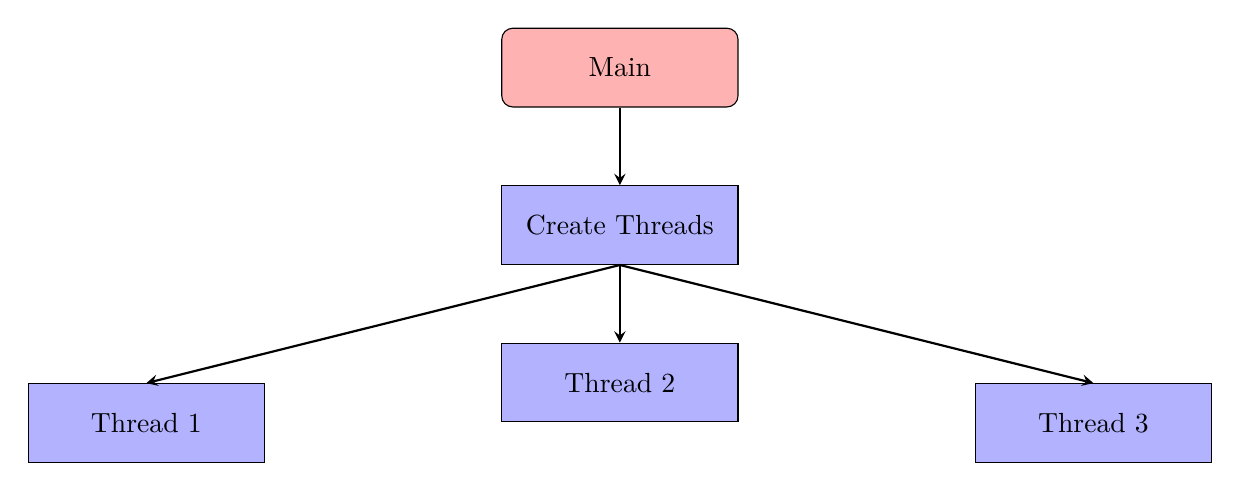
\begin{tikzpicture}[node distance=2cm]

    % Nodes
    \node (main) [startstop] {Main};
    \node (create) [process, below of=main] {Create Threads};
    
    % Threads
    \node (thread1) [process, below left=1.5cm and 3cm of create] {Thread 1};
    \node (thread2) [process, below of=create] {Thread 2};
    \node (thread3) [process, below right=1.5cm and 3cm of create] {Thread 3};
    
    % Arrows
    \draw [arrow] (main) -- (create);
    \draw [arrow] (create.south) -- (thread1.north);
    \draw [arrow] (create) -- (thread2.north);
    \draw [arrow] (create.south) -- (thread3.north);
    
\end{tikzpicture}
}
\end{center}

\columnbreak

\subsubsection*{创建多个 Socket}

我们可以考虑这样一种结构,将每一个发送请求接入服务端的 Client 都放置入一个线程当中,通过多线程的方式来实现多 Client 通信。
这里需要放在之前写的 \texttt{while} 循环当中,\texttt{pthread\_create()} 可以实现这个想法。
\end{multicols}

它的函数原型如下,其中需要提供一个函数指针,代表这个新建立的线程的函数入口。

\begin{mdframed}
    \textit{int pthread\_create(pthread\_t *thread, const pthread\_attr\_t *attr, void *(*start\_routine)(void *), void *arg);}
\end{mdframed}

查阅资料发现,\texttt{int pthread\_detach(pthread\_t thread);} 也有重要作用,具体如代码注释所述。

\begin{lstlisting}[language=C, title={Thread Creation}]
    while (1) {
        // 接受客户端连接
        client_socket = accept(server_socket, (struct sockaddr *)&client_addr, &client_addr_len);
        if (client_socket < 0) {
            perror("Accept failed");
            continue;
        }
        printf("New client connected.\n");

        // 创建线程处理客户端
        pthread_t thread_id;
        int *client_socket_ptr = malloc(sizeof(int));
        *client_socket_ptr = client_socket;

        if (pthread_create(&thread_id, NULL, client_handler, client_socket_ptr) != 0) {
            perror("Thread creation failed");
            free(client_socket_ptr);
            close(client_socket);
        }

        pthread_detach(thread_id); 
        // 这个函数是线程分离用的。将线程标记为分离状态。
        // 线程执行结束后系统会自动回收资源,无需通过 pthread_join() 等待线程结束。
        // 分离线程适用于短期任务,主线程不关心线程的返回值或执行状态。
    }
\end{lstlisting}

这里我们定义了 \texttt{client\_handler()} 函数作为线程的入口,它负责处理每个客户端的连接,可以把处理信息接受的逻辑放在这里:

另外要注意,我们要把各个 \texttt{client\_socket} 分开,所以采用了一个巧妙的设计:

\begin{ans}{}{}
\begin{itemize}
    \item 每个线程接收一个不同的指针 client\_socket\_ptr,指向各自动态分配的内存区域。
    \item *(int *)client\_socket\_ptr 提取该线程独立的套接字值。
    \item 调用 free(client\_socket\_ptr) 释放动态分配的内存,避免内存泄漏。
    \item 内存被释放后,每个线程内部仍然持有 client\_socket 的副本(值被解引用并存储在局部变量 client\_socket 中),互不影响。
\end{itemize}
\end{ans}

\begin{lstlisting}[language=C, title={Thread Handler}]
    //  POSIX 线程库的线程函数必须接受 void* 类型参数,因此需要强制转换。
    void *client_handler(void *client_socket_ptr) {
        int client_socket = *(int *)client_socket_ptr; // 动态分配内存,避免 client_socket 被覆盖
        free(client_socket_ptr);
    
        char buffer[MAX_LINE];
        ssize_t bytes_received;
    
        while (1) {
            memset(buffer, 0, sizeof(buffer)); // 接受消息之前,将缓存区清空,防止信息混乱
            bytes_received = recv(client_socket, buffer, sizeof(buffer) - 1, 0);
            // 确保保留最后一个字节给字符串的终止符 '\0',最后的参数 0 为标志位
            if (bytes_received <= 0) {
                printf("Client disconnected.\n");
                break;
            }
            printf("Received from client: %s\n", buffer);
        }
        close(client_socket);
    }
\end{lstlisting}

\begin{rmr}
至此,我们已经实现支持5个以上的 Client 同时发送消息并逐一打印!
\end{rmr}

\begin{figure}[H]
    \centering
    \includegraphics[width=0.9\linewidth]{lab7/multiclient.png}
    \caption{多客户端通信}
    \label{fig:multiclient}
\end{figure}

\subsection{Step 4: 实现从文件中读取}

在我的设计里,Client 进入了连接 Server 的状态后,是一直处于 \texttt{">"} 读取用户输入流的。

所以,只需要在输入流中检测是否出现 \textbf{FILE:}字段,并且读取后面跟随的文件名,再使用函数 \texttt{fopen()} 打开文件,并将文件内容发送给 Server 即可。

上面实现的逻辑很简单,可是应该怎样从文件中读取非常大的文本内容呢?

\subsubsection*{优化思路}

我们可以考虑使用 \texttt{fread()} 函数来逐块读取文件内容,并逐块发送给 Server。

\begin{ctt}
    在函数 \texttt{bytes\_read = fread(file\_buffer, 1, sizeof(file\_buffer), file);} 中:
    \begin{itemize}
        \item 第一个参数 file\_buffer 是用于存储读取数据的缓冲区。
        \item 第二个参数 1 是单个数据项的大小(字节数),这里是逐字节读取。
        \item 第三个参数 sizeof(file\_buffer) 是每次读取的最大数据项数,等于缓冲区大小(1024 字节)。
        \item fread 的返回值是实际读取到的字节数。
    \end{itemize}
\end{ctt}

\begin{lstlisting}[language=C, title={Read from File}]
    char file_buffer[1024]; 定义分块大小
    size_t bytes_read;
    while ((bytes_read = fread(file_buffer, 1, sizeof(file_buffer), file)) > 0) {
        ssize_t bytes_sent = send(client_socket, file_buffer, bytes_read, 0); // 逐块发送文件内容
        // 循环读取文件内容,直到文件结束(fread 返回值小于缓冲区大小或为 0)。
        if (bytes_sent < 0) {
            perror("Failed to send file");
            break;
        }
    }
\end{lstlisting}

\subsubsection*{完整代码}

根据上述的分析,我们可以将这部分判断是否需要从文件中读取的代码放在主循环中。

\begin{lstlisting}[language=C, title={Read from File}]
    while (1) {
        memset(buffer, 0, sizeof(buffer));
        printf("> ");
        fflush(stdout); // 刷新缓冲区,确保提示符显示
        read_input(buffer); // 读取输入

        // 如果是从文件中读取文本发送
        if (strncmp(buffer, "FILE:", 5) == 0) {
            char filename[MAX_LINE];
            sscanf(buffer + 5, "%s", filename); // 提取文件名

            FILE *file = fopen(filename, "r");
            if (!file) {
                perror("Failed to open file");
                continue;
            }

            // 从文件中读取文本并发送
            char file_buffer[1024];
            size_t bytes_read;
            while ((bytes_read = fread(file_buffer, 1, sizeof(file_buffer), file)) > 0) {
                ssize_t bytes_sent = send(client_socket, file_buffer, bytes_read, 0); // 逐块发送文件内容
                if (bytes_sent < 0) {
                    perror("Failed to send file");
                    break;
                }
            }
            fclose(file);
            printf("Text from file %s sent successfully.\n", filename);
        } else {
            // 否则,发送普通消息
            size_t total_sent = 0;
            size_t message_length = strlen(buffer);
            while (total_sent < message_length) {
                ssize_t bytes_sent = send(client_socket, buffer + total_sent, message_length - total_sent, 0);
                if (bytes_sent < 0) {
                    perror("Failed to send message");
                    break;
                }
                total_sent += bytes_sent;
            }
        }
    }
\end{lstlisting}

\subsubsection*{文件部分结果}

简单的文件传输已经获得了实现,如下所示:

\begin{figure}[H]
    \centering
    \includegraphics[width=0.9\linewidth]{lab7/file.png}
    \caption{从文件中读取}
    \label{fig:file}
\end{figure}

我采用实验资源包中提供的 test.txt 文件进行测试,文件大小为 21 KB,我将其命名为 long.txt 并放在服务器端的当前目录下。

大于 20 KB 的文件数据读取并进行通信的效果如下所示:

\begin{figure}[H]
    \centering
    \includegraphics[width=0.75\linewidth]{lab7/longtext.png}
    \caption{从文件中读取}
    \label{fig:long}
\end{figure}

\begin{rmr}
至此,我们已经实现 Client 能从标准输入或\textbf{文件}中接受消息。
\end{rmr}
\subsection{Step 5: 实现双工通信(客户端)}

考虑到实际上,在服务端同时接收多个客户端的信息时,实际上采用的是多个线程来处理的。

那么我们可以在每一个创建的 Client 中,新建一个线程来循环检测并接收服务端发来的信息。这样就能够实现双工通信了。

\begin{figure}[H]
    \centering
    \includegraphics[width=0.35\linewidth]{lab7/double.png}
    \caption{双工通信}
    \label{fig:fullduplex}
\end{figure}

因为在这边当 $n = 0$ 时,代表了服务端关闭,所以我们可以顺着实现一个功能:在服务端关闭时,发送一条消息给客户端,提示服务端已经关闭。

\begin{lstlisting}[language=C, title={Client Duplex}]
    typedef struct {
        int sockfd;
    } thread_args_t;
    
    // 接收线程函数:持续从服务器接收消息并打印
    void *recv_thread_func(void *arg) {
        thread_args_t *targs = (thread_args_t *)arg;
        int sockfd = targs->sockfd; // 获取套接字描述符
        char recv_buffer[1024];
        ssize_t n;
    
        while (1) {
            memset(recv_buffer, 0, sizeof(recv_buffer));
            n = recv(sockfd, recv_buffer, sizeof(recv_buffer) - 1, 0); // 0 表示阻塞接收模式
            // 返回值为 0,表示服务器关闭了连接
            if (n <= 0) {
                if (n < 0) {
                    fprintf(stderr, "Error receiving message: %s\n", strerror(errno));
                } else {
                    fprintf(stderr, "Server closed connection.\n");
                }
                break;
            }
            printf("\n[Message from server]: %s\n> ", recv_buffer);
            fflush(stdout);
        }
        return NULL;
    }
\end{lstlisting}

以上是该新建的线程从服务端不断接收消息并打印的函数,接下来我们只需要在 main 函数中,在连接到服务器之后创建该线程即可。

由于线程函数 \texttt{recv\_thread\_func} 的参数是 void *,只能传递单个指针,使用结构体封装参数能够传递多个值。

\begin{lstlisting}[language=C, title={Client Duplex}]
    pthread_t recv_tid;
    thread_args_t targs;
    targs.sockfd = client_socket; // 传递套接字描述符
    if (pthread_create(&recv_tid, NULL, recv_thread_func, &targs) != 0) {
        fprintf(stderr, "Create receive thread failed: %s\n", strerror(errno));
        close(client_socket);
        exit(EXIT_FAILURE);
    }
    pthread_detach(recv_tid);
\end{lstlisting}

\subsection{Step 6: 实现双工通信(服务端)}

我初步的设定是,在获得每一个 Client 发送的消息之后,添加消息回显(如时间戳等),这是很经典的双工通信的实现样式。
这部分实现逻辑应该放置在之前写的 \texttt{client\_handler()} 函数中,因为是回显给对应发送过来的客户端的,而非广播。

\begin{lstlisting}[language=C, title={Server Duplex}]
    #include<time.h>

    // 获取当前时间
    time_t now = time(NULL);
    struct tm *t = localtime(&now);
    char time_str[64];
    strftime(time_str, sizeof(time_str)-1, "%Y-%m-%d %H:%M:%S", t);

    // 构造回复消息
    char reply[MAX_LINE];
    snprintf(reply, sizeof(reply), "Server received your message: \"%s\" at %s\n", buffer, time_str);

    // 发送回复消息给客户端
    ssize_t bytes_sent = send(client_socket, reply, strlen(reply), 0);
    if (bytes_sent < 0) {
        perror("Send response message failed");
        break;
    }
\end{lstlisting}

\subsubsection*{实现结果图}

可以看到,创建了多个客户端,并且客户端在发送消息至服务端时,服务端会回显消息。服务器使用 Ctrl + C 中断关闭时,所有已连接到服务端的客户端都会显示“Server closed connection”信息。

\begin{figure}[H]
    \centering
    \includegraphics[width=0.7\linewidth]{lab7/fulldup.png}
    \caption{双工通信}
    \label{fig:fullduplex}
\end{figure}

\subsection{Step 7: 动态端口监听}

之前我们是把端口写死的(12345),而实验要求中需要将端口作为一个参数来传递。

\begin{lstlisting} [language=C]
    // 服务端的修改
    #define DEFAULT_SERVER_PORT 12345 // 我们先设置一个默认的端口,当命令行没有传入时就用这个
    int main(int argc, char *argv[]) {
        int server_port = DEFAULT_SERVER_PORT;
        // 解析命令行参数
        if (argc == 2) {
            server_port = atoi(argv[1]);
            if (server_port <= 0 || server_port > 65535) {
                fprintf(stderr, "Invalid port number: %s\n", argv[1]);
                exit(EXIT_FAILURE);
            }
        } else if (argc > 2) {
            fprintf(stderr, "Usage: %s [port]\n", argv[0]);
            exit(EXIT_FAILURE);
        }
    }
\end{lstlisting}

\begin{lstlisting} [language=C]
    // 客户端的修改
    #define DEFAULT_SERVER_PORT 12345
    int main(int argc, char *argv[]) {
        int server_port = DEFAULT_SERVER_PORT;
        char *server_ip;
        if (argc == 3) {
            server_ip = argv[1];
            server_port = atoi(argv[2]);
            if (server_port <= 0 || server_port > 65535) {
                fprintf(stderr, "Invalid port number: %s\n", argv[2]);
                exit(EXIT_FAILURE);
            }
        } else {
            fprintf(stderr, "Usage: %s <server_ip> <server_port>\n", argv[0]);
            exit(EXIT_FAILURE);
        }
    }
\end{lstlisting}

注意到,当右下角的客户端试图连接到 26420 端口时,会提示此时 Connection Refuse。

\begin{figure}[H]
    \centering
    \includegraphics[width=0.7\linewidth]{lab7/dynamicport.png}
    \caption{动态端口}
    \label{fig:dynamicport}
\end{figure}

\begin{rmr}
    目前,我们已经实现了:

    \begin{itemize} 
        \item 实现了多客户端与服务端之间的双工通信
        \item 实现了动态端口监听
        \item 连接到错误端口时会输出提示信息
    \end{itemize}

\end{rmr}

\subsection{Step Final: 优化细节}

\subsubsection{通过 fflush 优化缓冲区}

立即清除缓冲区,可以使得提示符马上显示:

\begin{lstlisting}[language=C, title={fflush}]
    printf("> ");
    fflush(stdout); // 清空缓冲区,立即显示提示符
\end{lstlisting}

\subsubsection{使用地址复用防止报错}

SO\_REUSEADDR 是套接字的一个选项,用于允许重新绑定地址,即使之前的连接还未完全关闭。

在 TCP 协议中,当关闭一个套接字后,连接可能会进入 TIME\_WAIT 状态(通常持续 1-4 分钟)。
在 TIME\_WAIT 状态下,该端口的地址仍被占用,导致重新启动服务器时,绑定同一端口会报错。

我们可以在创建 Socket 之后进行设置地址复用,解决这个问题。

\begin{lstlisting}[language=C, title={Address Reuse}]
    // 创建Socket
    if ((server_socket = socket(AF_INET, SOCK_STREAM, 0)) < 0) {
        perror("Socket creation failed");
        exit(EXIT_FAILURE);
    }

    // 复用地址避免重启服务器时的"Address already in use"
    int opt = 1;
    setsockopt(server_addr, SOL_SOCKET, SO_REUSEADDR, &opt, sizeof(opt));
\end{lstlisting}

\subsubsection{杀死服务端时关闭 Client}

在服务端使用 Ctrl + C 关闭时,只是关闭了 socket 连接,然而 Client 仍然还处于阻塞状态,这是由于不断读取消息的 while 循环导致的。

所以本来写的 \textbf{while(1)} 我想更换为 \textbf{while(running)},通过设置一个标志位来保证客户端程序的退出。

所有的 while 循环中都加入一个 running 的判断条件,就可以避免阻塞。

\begin{lstlisting}[language = C, title={Kill Client}]
volatile sig_atomic_t running = 1;  // 全局标志变量,用于控制主线程的退出

// 客户端修改位置:
if (n <= 0) {
    if (n < 0) {
        fprintf(stderr, "Error receiving message: %s\n", strerror(errno));
    } else {
        fprintf(stderr, "Server closed connection.\n");
    }
    running = 0; // 设置全局标志变量为 0,通知主线程退出
    close(sockfd); // 关闭套接字
    break;
}

while (running) {
    if {
        // 判断是使用文字输入还是文件输入,并发送消息
    }
    close(client_socket);
    return 0;
}
\end{lstlisting}

\subsubsection{优化客户端连接}

connect 函数会阻塞,直到成功连接到目标地址或发生错误(如超时或拒绝连接)。
如果输入的是一个无效的 IP 地址(如 asas),或者是一个无法路由的地址,connect 会一直等待。

所以我们可以添加一个连接超时的设置,这样使得客户端在连接到不对的 IP 地址时,过了指定的时间就会自动退出。

因为有时候我们也有使用域名进行连接的需求,而非简单的 IP 地址,这时候可以使用 \texttt{netdb.h} 库中的 \textbf{getaddrinfo} 来实现这个需求。

\begin{lstlisting}[language=C, title={Connect}]
    # include <netdb.h>

    // 使用 getaddrinfo 解析域名或 IP 地址
    struct addrinfo hints, *res;
    memset(&hints, 0, sizeof(hints));
    hints.ai_family = AF_INET;       // IPv4
    hints.ai_socktype = SOCK_STREAM; // TCP

    int ret = getaddrinfo(server_ip, NULL, &hints, &res);
    if (ret != 0) {
        fprintf(stderr, "getaddrinfo error: %s\n", gai_strerror(ret));
        close(client_socket);
        exit(EXIT_FAILURE);
    }

    struct sockaddr_in *addr_in = (struct sockaddr_in *)res->ai_addr;
    server_addr.sin_family = AF_INET;
    server_addr.sin_addr = addr_in->sin_addr;
    server_addr.sin_port = htons(server_port);

    freeaddrinfo(res);

    struct timeval timeout;
    timeout.tv_sec = 3; // 超时时间为 3 秒
    timeout.tv_usec = 0;
    setsockopt(client_socket, SOL_SOCKET, SO_SNDTIMEO, &timeout, sizeof(timeout));
    // 这里只设置发送的超时时间,不要设置接收的 SO_REVTIMEO 超时,否则连接上了也会断开

    // 尝试连接
    if (connect(client_socket, (struct sockaddr *)&server_addr, sizeof(server_addr)) < 0) {
    ...
    }
\end{lstlisting}

\begin{figure}[H]
    \centering
    \includegraphics[width=0.9\linewidth]{lab7/addr.png}
    \caption{连接超时提示}
    \label{fig:timeout}
\end{figure}

\subsection{Step More: 实现广播功能}

在服务端中,我们可以维护一个 Client 列表,当收到任意一个 Client 的 Broadcast 请求时,广播该信息到所有已连接到此处的客户端:

\begin{lstlisting}[language=C, title={Server Broadcast}]
// 全局客户端列表
int client_sockets[MAX_CLIENTS];
pthread_mutex_t client_list_mutex = PTHREAD_MUTEX_INITIALIZER;

// 广播功能的实现
void broadcast_message(const char *message) {
    pthread_mutex_lock(&client_list_mutex); // 加锁,避免并发修改客户端列表

    for (int i = 0; i < MAX_CLIENTS; i++) {
        if (client_sockets[i] != 0) {
            ssize_t bytes_sent = send(client_sockets[i], message, strlen(message), 0);
            if (bytes_sent < 0) {
                perror("Failed to send message to client");
            }
        }
    }

    pthread_mutex_unlock(&client_list_mutex); // 解锁
}

// 客户端连接时,加入列表中 
pthread_mutex_lock(&client_list_mutex);
for (int i = 0; i < MAX_CLIENTS; i++) {
    if (client_sockets[i] == 0) {
        client_sockets[i] = client_socket;
        break;
    }
}
pthread_mutex_unlock(&client_list_mutex);

// 客户端若已断开连接,从列表中移除
pthread_mutex_lock(&client_list_mutex);
for (int i = 0; i < MAX_CLIENTS; i++) {
    if (client_sockets[i] == client_socket) {
        client_sockets[i] = 0;
        break;
    }
}
pthread_mutex_unlock(&client_list_mutex);

\end{lstlisting}

\section{实验结果展示}

\begin{ctt}
    \begin{itemize}
    \item 连接至错误的 IP 地址 / 端口号时能提示出错信息 
    \item 能在标准输出打印客户端发送的消息
    \item 标准输入消息以两次回车为结束标志
    \end{itemize}
\end{ctt}

\begin{figure}[H]
    \centering
    \includegraphics[width=0.9\linewidth]{lab7/result.png}
\end{figure}

\begin{ctt}
    \begin{itemize}
    \item 绑定至错误的端口号时能提示出错信息
    \item 能从标准输入或文件中接收消息
    \item 支持 5 个以上客户端同时发送消息并逐一打印
    \item 支持长文本消息,有缓冲区管理
    \end{itemize}
\end{ctt}

\begin{figure}[H]
    \centering
    \includegraphics[width=0.9\linewidth]{lab7/result1.png}
\end{figure}

\begin{ctt}
    \begin{itemize}
        \item 能从标准输入或文件中接收消息
        \item 支持长文本消息,有缓冲区管理
    \end{itemize}
\end{ctt}

\begin{figure}[H]
    \centering
    \includegraphics[width=0.9\linewidth]{lab7/result2.png}
\end{figure}

其中,使用 \texttt{ls} 命令可以查看文件的大小:

\begin{figure}[H]
    \centering
    \includegraphics[width=0.9\linewidth]{lab7/filesize.png}
\end{figure}

\begin{ctt}
    \begin{itemize}
        \item 容错性好,无闪退 
        \item 支持双工通信
    \end{itemize}
\end{ctt}

服务端不仅可以接收到客户端的消息,还能及时反馈一条消息告诉客户端现在收到消息的时间戳。

同时,我还添加了服务端向客户端广播的功能,如果一个客户端想要发送广播给其他客户端,使用 \textbf{BROADCAST:} 命令即可。

\begin{figure}[H]
    \centering
    \includegraphics[width=0.9\linewidth]{lab7/result3.png}
\end{figure}

\begin{ctt}
    \begin{itemize}
        \item 支持在 localhost 和不同机器上运行
    \end{itemize}
\end{ctt}

我使用我的另一台电脑安装了适用于 WSL 的 Windows 子系统,在这里编译使用了我编写的代码,成功运行。

\begin{figure}[H]
    \centering
    \includegraphics[width=0.7\linewidth]{lab7/secondpc.png}
\end{figure}

\begin{figure}[H]
    \centering
    \includegraphics[width=0.95\linewidth]{lab7/run.png}
\end{figure}

\renewcommand{\arraystretch}{1.5} % 调整行间距
\setlength{\tabcolsep}{6pt} % 调整列间距

\begin{table}[H]
\centering
\resizebox{0.5\textwidth}{!}{
\begin{tabular}{|m{6cm}<{\centering}|m{6cm}<{\centering}|}
\hline
\textbf{能在标准输出打印客户端发送的消息(20分)} & \textbf{支持5个以上客户端同时发送消息并逐一打印(20分)} \\ \hline
\ding{51} & \ding{51} \\ \hline
\textbf{能从标准输入或文件接收消息(20分)} & \textbf{标准输入消息以两次回车作为结束标志(5分)} \\ \hline
\ding{51} & \ding{51} \\ \hline
\textbf{绑定至错误的端口号时能提示出错信息(5分)} & \textbf{连接至错误的IP地址/端口号时能提示出错信息(5分)} \\ \hline
\ding{51} & \ding{51} \\ \hline
\textbf{支持在 localhost 及在两台不同机器上运行(10分)} & \textbf{支持长文本消息(不少于 20KB),有缓冲区管理(10分)} \\ \hline
\ding{51} & \ding{51} \\ \hline
\textbf{容错性好,无闪退(5分)} & \textbf{支持双工通信(5分)} \\ \hline
\ding{51} & \ding{51} \\ \hline
\end{tabular}
}
\caption{评分表}
\end{table}

\subsection{编译指南}

由于我们已经实现了全双工通信,此时用到了多线程处理,因此需要使用 pthread 库。
按照\href{http://staff.ustc.edu.cn/~mengning/np/linux_socket/new_page_4.htm}{中国科学技术大学的 Linux Socket 编程指南},
我们需要在最后添加 -lthread 编译选项:

依次使用以下命令:

\begin{lstlisting}
    $ gcc -o client client.c -lpthread
    $ gcc -o server server.c -lpthread
\end{lstlisting}

\begin{ctt}
    后来我发现,在我的主电脑上,其实不加也可以...应该是因为某些 Linux 正式发行版中已经预置了常用了链接库。
    
    但是在我的副电脑上编译时,如果不加入这个参数就会报链接错误。
\end{ctt}

\subsection{运行指南}

\begin{lstlisting}
    > ./server [port]
\end{lstlisting}

\begin{lstlisting}
    > ./client <server_ip> <server_port> or > ./client localhost <server_port>
    > FILE:<file_name> # 需要加后缀
    > BROADCAST:<message> # 发送广播消息
\end{lstlisting}

\section{附录}

\subsection{参考资料}

\begin{itemize}
    \item 中科大 Linux Socket 编程指南:\href{http://staff.ustc.edu.cn/~mengning/np/linux_socket/new_page_4.htm}{\underline{http://staff.ustc.edu.cn/~mengning/np/linux\_socket/new\_page\_4.htm}}
    \item Linux Manual Page:\href{https://man7.org/linux/man-pages/man7/pthreads.7.html}{\underline{https://man7.org/linux/man-pages/man7/pthreads.7.html}}
\end{itemize}

\subsection{完整代码}

\subsubsection{客户端代码(client.c)}

\begin{lstlisting}[language=C]
    #include <stdio.h>
    #include <stdlib.h>
    #include <string.h>
    #include <strings.h>
    #include <unistd.h>
    #include <arpa/inet.h>
    #include <errno.h>
    #include <signal.h>
    #include <pthread.h>
    #include <netdb.h> // for getaddrinfo
    
    #define DEFAULT_SERVER_PORT 12345
    #define MAX_LINE 20480
    
    typedef struct {
        int sockfd;
    } thread_args_t;
    
    volatile sig_atomic_t running = 1; // 全局标志变量,用于控制主线程的退出
    
    // 接收线程函数:持续从服务器接收消息并打印
    void *recv_thread_func(void *arg) {
        thread_args_t *targs = (thread_args_t *)arg;
        int sockfd = targs->sockfd; // 获取套接字描述符
        char recv_buffer[1024];
        ssize_t n;
    
        while (running) {
            memset(recv_buffer, 0, sizeof(recv_buffer));
            n = recv(sockfd, recv_buffer, sizeof(recv_buffer) - 1, 0); // 0 表示阻塞接收模式
            // 返回值为 0,表示服务器关闭了连接
            if (n <= 0) {
                if (n < 0) {
                    fprintf(stderr, "Error receiving message: %s\n", strerror(errno));
                } else {
                    fprintf(stderr, "Server closed connection.\n Input anything and <Enter> to exit.");
                }
                running = 0;
                close(sockfd);
                exit(EXIT_SUCCESS);
            }
            printf("\n[Message from server]: %s\n> ", recv_buffer);
            fflush(stdout);
        }
        return NULL;
    }
    
    // 从标准输入读取消息,直到两个回车为结束标志
    void read_input(char *buffer) {
        char temp[MAX_LINE];
        int idx = 0;
        while (fgets(temp, sizeof(temp), stdin) && (running)) { // 从标准输入流中读取
            // 如果是连续两个回车,移除最后一个回车,保证字符串正确
            if (strcmp(temp, "\n") == 0 && idx > 0 && buffer[idx - 1] == '\n') {
                buffer[idx - 1] = '\0'; // 移除最后一个回车
                return;                 // 此时可以 return,代表结束标志
            }
    
            // 如果一行里输入得太长了,报错并退出
            if (idx + strlen(temp) >= MAX_LINE) {
                fprintf(stderr, "Input too large.\n");
                exit(EXIT_FAILURE);
            }
            strcpy(buffer + idx, temp); // 追加本行内容到 buffer 数组中
            idx += strlen(temp);
        }
    }
    
    int main(int argc, char *argv[]) {
        int client_socket;
        struct sockaddr_in server_addr;
        char buffer[MAX_LINE];
        int server_port = DEFAULT_SERVER_PORT;
        char *server_ip;
    
        if (argc == 3) {
            server_ip = argv[1];
            server_port = atoi(argv[2]);
            if (server_port <= 0 || server_port > 65535) {
                fprintf(stderr, "Invalid server port: %s\n", argv[2]);
                exit(EXIT_FAILURE);
            }
        }
        else {
            fprintf(stderr, "Usage: %s <server_ip> <server_port>\n", argv[0]);
            exit(EXIT_FAILURE);
        }
    
        // 创建Socket
        if ((client_socket = socket(AF_INET, SOCK_STREAM, 0)) < 0) {
            perror("Socket creation failed");
            exit(EXIT_FAILURE);
        }
    
        // 使用 getaddrinfo 解析域名或 IP 地址
        struct addrinfo hints, *res;
        memset(&hints, 0, sizeof(hints));
        hints.ai_family = AF_INET;       // IPv4
        hints.ai_socktype = SOCK_STREAM; // TCP
    
        int ret = getaddrinfo(server_ip, NULL, &hints, &res);
        if (ret != 0)
        {
            fprintf(stderr, "getaddrinfo error: %s\n", gai_strerror(ret));
            close(client_socket);
            exit(EXIT_FAILURE);
        }
    
        struct sockaddr_in *addr_in = (struct sockaddr_in *)res->ai_addr;
        server_addr.sin_family = AF_INET;
        server_addr.sin_addr = addr_in->sin_addr;
        server_addr.sin_port = htons(server_port);
    
        freeaddrinfo(res);
    
        // 设置连接超时
        struct timeval timeout;
        timeout.tv_sec = 3; // 超时时间为 5 秒
        timeout.tv_usec = 0;
        setsockopt(client_socket, SOL_SOCKET, SO_SNDTIMEO, &timeout, sizeof(timeout));
        // 这里只设置发送的超时时间,不要设置接收的 SO_REVTIMEO 超时,否则连接上了也会断开
    
        // 尝试连接
        if (connect(client_socket, (struct sockaddr *)&server_addr, sizeof(server_addr)) < 0) {
            perror("Connection failed");
            close(client_socket);
            exit(EXIT_FAILURE);
        }
    
        printf("Connected to server %s:%d.\n. Enter your message (end with double ENTER):\n", server_ip, server_port);
    
        // 创建接收线程
        pthread_t recv_tid;
        thread_args_t targs;
        targs.sockfd = client_socket;
        if (pthread_create(&recv_tid, NULL, recv_thread_func, &targs) != 0)
        {
            fprintf(stderr, "Creating receive thread failed: %s\n", strerror(errno));
            close(client_socket);
            exit(EXIT_FAILURE);
        }
        pthread_detach(recv_tid);
    
        // 主循环:读取输入并发送消息
        while (running) {
            memset(buffer, 0, sizeof(buffer));
            printf("> ");
            fflush(stdout); // 刷新缓冲区,确保提示符显示
            read_input(buffer); // 读取输入
    
            // 如果是从文件中读取文本发送
            if (strncmp(buffer, "FILE:", 5) == 0) {
                char filename[MAX_LINE];
                sscanf(buffer + 5, "%s", filename); // 提取文件名
    
                FILE *file = fopen(filename, "r");
                if (!file) {
                    perror("Failed to open file");
                    continue;
                }
    
                // 从文件中读取文本并发送
                char file_buffer[1024];
                size_t bytes_read;
                while (((bytes_read = fread(file_buffer, 1, sizeof(file_buffer), file)) > 0) && (running)) {
                    ssize_t bytes_sent = send(client_socket, file_buffer, bytes_read, 0); // 逐块发送文件内容
                    if (bytes_sent < 0) {
                        perror("Failed to send file");
                        break;
                    }
                }
                fclose(file);
                printf("Text from file %s sent successfully.\n", filename);
            } else {
                // 否则,发送普通消息
                size_t total_sent = 0;
                size_t message_length = strlen(buffer);
                while ((total_sent < message_length) && (running)) {
                    ssize_t bytes_sent = send(client_socket, buffer + total_sent, message_length - total_sent, 0);
                    if (bytes_sent < 0) {
                        perror("Failed to send message");
                        break;
                    }
                    total_sent += bytes_sent;
                }
            }
        }
    
        close(client_socket);
        return 0;
    }    
\end{lstlisting}

\subsubsection{服务器代码(server.c)}

\begin{lstlisting}[language=C]
    #include <stdio.h>
    #include <stdlib.h>
    #include <string.h>
    #include <strings.h>
    #include <unistd.h>
    #include <pthread.h>
    #include <arpa/inet.h>
    
    #define DEFAULT_SERVER_PORT 12345
    #define MAX_LINE 20480 // 支持长文本消息
    #define MAX_PENDING 5
    #define MAX_CLIENTS 10
    
    // 客户端套接字列表和互斥锁
    int client_sockets[MAX_CLIENTS];
    pthread_mutex_t client_list_mutex = PTHREAD_MUTEX_INITIALIZER;
    
    // 处理广播消息的函数
    void broadcast_message(const char *message)
    {
        pthread_mutex_lock(&client_list_mutex); // 加锁,避免并发修改客户端列表
    
        for (int i = 0; i < MAX_CLIENTS; i++)
        {
            if (client_sockets[i] != 0)
            {
                ssize_t bytes_sent = send(client_sockets[i], message, strlen(message), 0);
                if (bytes_sent < 0)
                {
                    perror("Failed to send message to client");
                }
            }
        }
    
        pthread_mutex_unlock(&client_list_mutex); // 解锁
    }
    
    //  POSIX 线程库的线程函数必须接受 void* 类型参数,因此需要强制转换。
    void *client_handler(void *client_socket_ptr) {
        int client_socket = *(int *)client_socket_ptr; // 动态分配内存,避免 client_socket 被覆盖
        free(client_socket_ptr);
    
        char buffer[MAX_LINE];
        ssize_t bytes_received;
    
        // 将客户端加入到客户端列表
        pthread_mutex_lock(&client_list_mutex);
        for (int i = 0; i < MAX_CLIENTS; i++) {
            if (client_sockets[i] == 0) {
                client_sockets[i] = client_socket;
                break;
            }
        }
        pthread_mutex_unlock(&client_list_mutex);
    
        while (1) {
            memset(buffer, 0, sizeof(buffer)); // 接受消息之前,将缓存区清空,防止信息混乱
            bytes_received = recv(client_socket, buffer, sizeof(buffer) - 1, 0);
            // 确保保留最后一个字节给字符串的终止符 '\0',最后的参数 0 为标志位
            if (bytes_received <= 0) {
                printf("Client disconnected.\n");
    
                // 客户端断开连接时,从客户端列表中移除
                pthread_mutex_lock(&client_list_mutex);
                for (int i = 0; i < MAX_CLIENTS; i++)
                {
                    if (client_sockets[i] == client_socket)
                    {
                        client_sockets[i] = 0;
                        break;
                    }
                }
                pthread_mutex_unlock(&client_list_mutex);
    
                break;
            }
            printf("Received from client: %s\n", buffer);
    
            // 检查是否是广播命令
            if (strncmp(buffer, "BROADCAST:", 10) == 0) {
                char *message = buffer + 10; // 跳过 "broadcast:" 部分
                broadcast_message(message);  // 广播消息
            } else {
                // 获取当前时间
                time_t now = time(NULL);
                struct tm *t = localtime(&now);
                char time_str[64];
                strftime(time_str, sizeof(time_str) - 1, "%Y-%m-%d %H:%M:%S", t);
    
                // 构造回复消息
                char reply[MAX_LINE];
                snprintf(reply, sizeof(reply), "Server received your message at %s\n", time_str);
    
                // 发送回复消息给客户端
                ssize_t bytes_sent = send(client_socket, reply, strlen(reply), 0);
                if (bytes_sent < 0) {
                    perror("Send response message failed");
                    break;
                }
            }
        }
    
        close(client_socket);
        return NULL;
    }
    
    int main(int argc, char *argv[]) {
        int server_socket, client_socket;
        struct sockaddr_in server_addr, client_addr;
        socklen_t client_addr_len = sizeof(client_addr);
        int server_port = DEFAULT_SERVER_PORT;
    
        // 解析命令行参数
        if (argc == 2) {
            server_port = atoi(argv[1]);
            if (server_port <= 0 || server_port > 65535) {
                fprintf(stderr, "Invalid port number: %s\n", argv[1]);
                exit(EXIT_FAILURE);
            }
        } else if (argc > 2) {
            fprintf(stderr, "Usage: %s [port]\n", argv[0]);
            exit(EXIT_FAILURE);
        }
    
        // 创建Socket
        if ((server_socket = socket(AF_INET, SOCK_STREAM, 0)) < 0) {
            perror("Socket creation failed");
            exit(EXIT_FAILURE);
        }
    
        // 复用地址避免重启服务器时的"Address already in use"
        int opt = 1;
        setsockopt(server_socket, SOL_SOCKET, SO_REUSEADDR, &opt, sizeof(opt));
    
        // 配置服务器地址
        bzero((char *)&server_addr, sizeof(server_addr));
        server_addr.sin_family = AF_INET;
        server_addr.sin_addr.s_addr = INADDR_ANY;
        server_addr.sin_port = htons(server_port);
    
        // 绑定Socket
        if (bind(server_socket, (struct sockaddr *)&server_addr, sizeof(server_addr)) < 0) {
            perror("Bind failed");
            close(server_socket);
            exit(EXIT_FAILURE);
        }
    
        // 监听连接
        if (listen(server_socket, MAX_PENDING) < 0) {
            perror("Listen failed");
            close(server_socket);
            exit(EXIT_FAILURE);
        }
    
        printf("Server is listening on port %d\n", server_port);
    
        while (1) {
            // 接受客户端连接
            client_socket = accept(server_socket, (struct sockaddr *)&client_addr, &client_addr_len);
            if (client_socket < 0) {
                perror("Accept failed");
                continue;
            }
            printf("New client connected.\n");
    
            // 创建线程处理客户端
            pthread_t thread_id;
            int *client_socket_ptr = malloc(sizeof(int));
            *client_socket_ptr = client_socket;
    
            if (pthread_create(&thread_id, NULL, client_handler, client_socket_ptr) != 0) {
                perror("Thread creation failed");
                free(client_socket_ptr);
                close(client_socket);
            }
            pthread_detach(thread_id);
            // 这个函数是线程分离用的。将线程标记为分离状态。
            // 线程执行结束后系统会自动回收资源,无需通过 pthread_join() 等待线程结束。
            // 分离线程适用于短期任务,主线程不关心线程的返回值或执行状态。
        }
        close(server_socket);
        return 0;
    }    

\end{lstlisting}

\end{document}